\documentclass[12pt,letter]{article}
\usepackage[DIV=14,BCOR=2mm,headinclude=true,footinclude=false]{typearea}
\renewcommand{\baselinestretch}{1.15} 
\usepackage{latexsym}
\usepackage{amsmath}
\usepackage{MinionPro}
\usepackage{hyperref}
\usepackage{tikz}
\usepackage{verbatim}
\usepackage{natbib}
\usepackage{color, colortbl}
\usepackage{appendix}
\usepackage{amsmath,amsthm}

%\usepackage{mathptmx}
%\usepackage{MnSymbol}
%\usepackage{wasysym}
%\usepackage{amssymb}

\usetikzlibrary{arrows,shapes}

\definecolor{Gray}{gray}{0.9}

\newtheorem{result}{Result}
\newtheorem{theorem}{Theorem}[section]
\newtheorem{conjecture}{Conjecture}[section]
\newtheorem{corollary}{Corollary}[section]
\newtheorem{lemma}{Lemma}[subsection]
\newtheorem{proposition}{Proposition}[section]
\newtheorem{definition}{Definition}[section]
\newtheorem{assumption}{Assumption}[section]

\theoremstyle{remark}
\newtheorem{example}{Example}[section]

\theoremstyle{remark}
\newtheorem*{remark}{Remark}

\theoremstyle{claim}
\newtheorem*{claim}{Claim}

\pgfdeclarelayer{background}
\pgfsetlayers{background,main}

\tikzstyle{vertex}=[circle,fill=black!25,minimum size=12pt,inner sep=0pt]
\tikzstyle{selected vertex} = [vertex, fill=red!24]
\tikzstyle{edge} = [draw,thick,-]
\tikzstyle{weight} = [font=\small]
\tikzstyle{selected edge} = [draw,line width=5pt,-,red!50]
\tikzstyle{ignored edge} = [draw,line width=5pt,-,black!20]


%\linespread{1.5}

\begin{document}
%\fontsize{12}{20pt}\selectfont

\title {Coordination in Social Networks}
\author {by Chun-Ting Chen}

\maketitle

\begin{abstract}

This paper studies a coordination program in a repeated coordination game setting\footnote{with discounting}, in which players' private information is aligned with their positions in the social networks. Players only know their neighbors' inclinations in participation initially and can only monitor their neighbors' past actions. Given that the network is fixed, finite, undirected, and commonly known, the main result is to show that there is always a sequential equilibrium in which a stage game ex-post efficient participation level will eventually coordinated in every tree network when discounted factor is sufficient high.



\end{abstract}


\section{Introduction} 

This paper studies the collective action behaviour in a setting of repeated coordination games where information structure and monitoring structure is modelled as networks. I then ask what kinds of networks can induce people to solve the uncertainty about underlying relevant information and coordinate to the ex-post efficient outcome. Though the main motivation lies in understanding the dynamic of social movement, a general interest is in the interaction between collective action and social structure.

Consider people's anger in a rigid regime. A anger power against this regime may exist, but these powers are hard to put together due to the lack of complete information about this power and due to communication barrier to link this power. In the era of East German, the voting and mass media is controlled by the government and eavesdrop impede people shows their political discontent. Before 1911 in China, several underground forces against Ching Dynasty scattered on the southern of China, but they have different opinions in when and how to make a revolution, and the ways in communication is dangerous. Though some social network such as the networks of friends, of organizations, served as routes in communication, but the communication is not free but costly in the sense that it is risky. While Berlin Wall and Ching Dynasty become a history, we may then ask how such decisive protest (or revolution in China's case) overcome such information barrier and conduct its successfulness.

As social scientist has recognize it, the process of social movement can be traced back to periods ago, and an event may trigger another event. In game theory, a well-known feature in the extensive form incomplete information game is that the information set is evolved with players' actions, and so that players can use this additional information to explore the true state. When rebels know that their risky actions can be used to transmit relevant information about the potential power, they may be willing to take such actions in the hope that such power exists and other rebels know this power exists,...,and so on, and so that a decisive protest can be made successfully. Needless to say that a social movement always involves some sacrifices which may seems tiny and useless before its successfulness. I view such risky actions as parts of a equilibrium strategy and the entire movement as a learning process. 

Inspired by [Chwe], I model social network as a information structure. In this information structure, {both} of people's type and their actions can be observed {perfectly and only} by their neighbours. The network is fixed, finite, and commonly known. 

The static game is a simple version of ``$k$-\textit{Threshold game}'' [Chwe]. In this $k$-Threshold game, there are two types of players located in the network, one we called them \textit{Rebel} and one we called them \textit{Inert}. A state of nature is the product of players types. A Rebel has two actions, which are \textbf{revolt} or \textbf{stay}. A Inert has only one action, which is \textbf{Inert}. There is a parameter, $k\in \mathbb{N}$, which is relevant for Rebels' pay-off but not for Inerts. The pay-off is defined as the followings. 
\begin{enumerate}
\item If a Rebel chooses \textbf{revolt}, and there are more than $k$ people who \textbf{revolt}, then this Rebel will get a positive pay-off, simplified as $1$;
\item If a Rebel chooses \textbf{revolt}, but there are less than $k$ people who \textbf{revolt}, then this Rebel get negative pay-off, simplified  as $-1$;
\item If a Rebel choose \textbf{stay}, then he will get a pay-off, simplified as $0$ no matter how others play.
\item Inert always play \textbf{Inert}, and get a positive pay-off, simplified as $1$, no matter how others play. 
\end{enumerate}
Thus, Rebels play the game against all other players, but they certain about their neighbours' type and actions only. Because Inerts will not play \textbf{revolt}, Rebels' pay-off structure captures the idea that choosing \textbf{stay} is a safe action while choosing \textbf{revolt} will faces the uncertainty about others' types and others' plays. 

Given the threshold $k$ and a prior $\pi$, those rebels repeatedly play the $k$-Threshold game infinitely with a common discount factor $\delta$. The ways for communication is extremely restricted in the sense that cheap talks is not allowed, no outside mechanism serves as an information exchange device, and the static pay-off is unobservable.

The only way for Rebels to communicate with each other is to create the signals by their actions, which will incurs some risky actions. These signals created by Rebels' actions have to be parts of a sequential equilibrium. With various $k$ and various network structures, I am finding a sequential equilibrium which has a property of \textit{approaching ex-post efficient} no matter how prior $\pi$ is (or how prior which is within a large set of $\pi$s is) to investigate the interaction between network information structure and such information creation and sharing behaviour in conducting coordination. More precisely, we say a sequential equilibrium is approaching ex-post efficiency if the tails of actions in the equilibrium path repeats the ex-post efficient outcome in the underlying static game after a finite period. \footnote{Note that the definition of approaching ex-post efficiency consider the tails of actions in the path, but did not consider players' expected pay-off in the path.}. This concept mainly checking the in-path  behaviour in which players \text{seems} like they will learned the true state eventually no matter how the initial prior over states (or a large set of states) of nature is. In words, if there are at least $k$ Rebels in this society, then we shall see \textit{all} Rebels revolt in the future; otherwise, \textit{all} Rebels should stay in the future.

In the hope that the uncertainty of ``\textit{there are at least $k$ Rebels in this society}'' can be solved, Rebels may then have incentive to cooperate in creating signals and transmit such signals to reveal the state of ``\textit{total number of Rebels in this society}'' if they care future pay-off a lot. Such incentives is certainly affected by the network structure. This is because both incomplete information structure and monitoring structure are aligned with network here, and thus the information can be only transmitted via the edge. For example, if every Rebels are singletons, then there is no way to share their information. But more importantly, this incentive is affected by their position in the network. For example, if the network is a wheel, only center Rebel (if the center is a Rebel) can learn the true state and transmit such information to others by himself. If there is a cost to transmit such information, the Rebels connected to the center can be the free rider in some equilibrium, but the center will never be the free rider in a equilibrium.   

To get a quick intuition about the learning process, consider the case when $k=n$, and suppose the network is also connected and undirected. A simple contagion argument will get the following result.
\begin{result}
For $n$-person repeated $k$-Threshold game with parameter $k=n$ played in any fixed finite connected undirected network, if for each pairs of Rebels then there is a path full with Rebels connect them, then for any prior there is a $\delta$ such that there is a sequential equilibrium which is approaching ex-post efficient.
\end{result}

The argument to show the equilibrium path is to treat \textbf{stay} as the message of ``there is an Inert out there''; and treat \textbf{revolt} as the message of ``there could be no Inert out there ''. If I (a Rebel) have an Inert neighbour, then I play stay for ever. If I have no Inert neighbours, then I play revolt in this period. If I have saw my neighbour played stay, then I play stay for ever. If I have saw my neighbour played revolt, then I continue to play revolt. I can learn the true state in finite period because the network is finite and among other properties. One can then find a belief system and suitable off-path strategies to construct an equilibrium with approaching ex-post efficiency. 

The equilibrium construction in Result 1 is simple because these binary actions exactly partition the states into two parts, no Inerts or some Inerts, and that is a sufficient information Rebels need to know to make coordination when $k=n$. It is similar to the full-rank condition with which actions can generate distinguishable distribution of signals. However, when $1<k<n$, as we will show later, more information (or more dimensions of information, larger than $2$) needed to be carried by such binary actions. Several sequence of actions has to be used to transmit the information, and such sequences are better to be very clear in the sense that no mixed strategies to be used. Otherwise, the belief updating seems very intractable when the network become complicated.




The equilibrium is constructive and is written down as an automata. In the equilibrium path, two kinds of binary $\{\textbf{revolt},\textbf{inert}\}$-sequences has been used to control Rebels' beliefs. The first one, called it \textit{reporting sequences}, is to report the current information about $k$ to others, while the later one, called it \textit{coordination sequences}, is to answer the question of whether there is at least $k$ Rebels in the society. The reporting sequence then mean to control individual's belief about the number of $k$, and the usage of coordination sequence serves as short-cut by exploiting the assumption on network structure to bypass the tracking of individual's belief about others' belief about others' belief...about $k$\footnote{The major incentives to induce Rebels to reveal their information here is to give them some hope to coordinate to the ex-post efficient pay-off. It then require individual's growing confidence of the true number of Rebels out there, and individual's growing confidence of others' growing confidence of that, and so on. When the network getting complicated, it then seems intractable to keep track this giant belief profile.}. To see this, suppose at some periods, a Rebel has known the true number of $k$, then such Rebel can use this coordination message to notify nearby Rebels. Since the network is finite, undirected, there is a finite time to broadcast this knowledge entirely in the network. Then this knowledge will become ``public'' due to the network structure is commonly known, and then Rebels start coordination at this timing conditional on this message.


We then want players to share their information by using reporting sequence. However, the usage of this sequence is not free in the sense that every usage of action \textbf{revolt} is risky\footnote{Indeed, if we allow cheap talk, or we use limit-of-mean preference, or we already have a Folk theorem in this setting, then \textbf{Result 2} or \textbf{Result 3} will trivially hold. If we allow cheap talk (or limit-of-mean preference), then Rebels just use cheap talk (or their actions as messages) to talk about``how many Rebels are nearby them''. Players has no incentive to lie due to the game is a coordination game. As far as my knowledge, a Folk theorem has not proposed to cover my setting during the time when this paper is under working. }. Due to there is a discounting, if reporting more information incurs more (less) risky actions, then they have incentive to report less (more). As the problem will be cleared later, combined the usage of the coordination message and the sequential message (reporting or coordination) will incur a prisoner dilemma happened locally aligned with the network. Briefly speaking, suppose two nearby Rebels exchange information and true state can be revealed only by them, and suppose \textit{every} Rebel can use coordination message to trigger coordination \textit{no matter} how his/her past reporting message looks like, then both players will shrink by not reporting anything since they can wait for other's reporting, but then no one can learn the true state. Thus the acceptance of coordination triggered by coordination message should not be freely from the past reporting messages. We overcome this issue by tailoring the reporting messages and using a grim-trigger-like belief as a punishment.

The off-path belief serves as a ``Grim Trigger'': when a Rebel detect a deviation, she believe that all other persons outside her neighbours are all Inerts. This threat is credible when less than $k$ Rebels in her neighbourhood. This grim-trigger-like belief enforces Rebels' strategies follow a prescribed form in the equilibrium path since a deviation from the form can be detected and will be considered as deviation. However, it incurs another problem due to the the pay-off function is not continuous at the threshold of $k$ Rebels' revolts. A Rebel is more willing to share his information in the hope of $k$ Rebels' coordination before he knows there are enough $k$ Rebels, but is less willing to share his information after he has known since more Rebels' coordination did not change his pay-off.  Combined the effect of costly messages and the potential imperfect monitoring structure, a Rebel will then seek the opportunity to reduce his cost in transmitting messages by not transmit this information to others Rebels while this reduction did not affect the coordination made by existing $k$ Rebels he already known. The criteria in judging deviation in the path then should not be too strict , otherwise some rebels may be excluded from a coordination. \footnote{For example, suppose the acceptance of coordination requires the summation, my current information about the number of Rebels plus my neighbour's such information inferred by his reporting, exceeds threshold $k$. Due to the incomplete information and imperfect monitoring, my neighbour can report less but actually my neighbour has known the number of Rebels has exceed threshold. Later on, my neighbour trigger the coordination message to coordinate the neighbours on his right-handed side, but I did not join since my belief tell me no other Rebels outside my neighbourhood.}. 

I show that this coordination problem can be overcame in a tree network given that the network is fixed finite connected undirected, as Result 2 shows. However when the network is with circle, the question remains unsolved, although the equilibrium strategies mean to be tailored for solving it.  

\begin{result}
For $n$-person repeated $k$-Threshold game with parameter $1\leq k \leq n$ played in any fixed finite connected undirected network without cycle,
if the state has strong connectivity and $\Pi(\text{the states has strong connectivity})=1$, then there is a $\delta$ such that there is a sequential equilibrium which is approaching ex-post efficient.
\end{result}

\begin{result}
For $n$-person repeated $k$-Threshold game with parameter $1\leq k \leq n$ played in any fixed finite connected undirected network,
if the state has strong connectivity and $\pi[\text{the states has strong connectivity}]=1$, then there is a $\delta$ such that there is a sequential equilibrium which is approaching ex-post efficient.
\end{result}

The free rider problem may become more severe when a network has a cycle. If a network has no cycle, a result will show that the potential free rider problem only happen between at most two connected Rebels. I then use a rule to determine which Rebel can be a free rider and which one should transmit information to him. However, when a network has cycle, there is an example shows that this problem can happen among more Rebels, and these Rebels may not connected to each together. This problem will remain later to discuss.





 


 
In the equilibrium path, we make sure that the signals Rebels sent and Rebel received are very clean in the sense that each state will specify one unique sequence of action.




 



As Amitai has point out, not every incomplete information static game can be revealed its true state, when the internal conflict of interest issue exist in static game and when people can not reveal the true state \textit{simultaneously} due to the limitation of message space. 





 





 I did not mean to prove a folk theorem in this paper, while the most literature in folk theorem seem to search the conditions for games and information structure simultaneous, such as various full-rank conditions have been proposed to let all (or some) of individual rational pay-off points be sustainable. Since I did not vary the static game and the information structure simultaneous, the property of this static game is crucial in constructing equilibria.



   
 Though this special kind of network information structure is relatively seldom mentioned by current repeated game literature, the usage of network structure here is to capture the degree of What people known, What people have seen, and ``How far'' them have known and seen. When it is applied to the repeated game setting, the equilibrium behaviour will then capture this information transmitting in the time horizontal line. This social network is commonly know, fixed, finite, connected, undirected over time\footnote{It is hard to say this assumption is too strong or not,}.







“There are decades where nothing happens; and there are weeks where decades happen.” 




In reality, one can replace the term, revolution, by aggressive financial investment or co-working project, which need certain amount of input from individuals. 

Such feature of modelling is to view the network structure as an information structure.


Now I compare my model setting with the existing literature. The main difference is that the players are playing a repeated game in the network, which can be viewed as a far-sight learning protocol, while the existing literature concerning about learning in a network mainly state the problem as a decision problem (such as \cite{BG1998}, or \cite{GK2003}). In \cite{BG1998}, they let each individual has heterogeneous parameters about the prior, and let individual make one-period expected utility maximizations in each period. In \cite{GK2003}, they let individuals get a private signal (for instance, $\omega_i$) about the true state (for instance, $\omega_1,.\omega_i.,\omega_n$), while individuals' pay-off depends on some functions taken the value of true state (for instance $\sum^n_i\omega_i$). Each individual makes decision concerning about one-period expected utility, but did not concern about their decision strategically.  

I assume the network is undirected throughout this paper. In \cite{BG1998}, they put the same assumption on their model, and then got an important insight in their results. With assuming that individuals' can observe their neighbours' one-period outcome in each period, if the network is connected and undirected, each individual get the same expected utility in the long-run. This is because an individuals can always mimic their neighbours' decisions since the network is undirected, and a connected network will spread these decisions over the whole communities. Since the goal of this paper is to find the successful coordination (ex-post efficient) in the long-run, I put the same assumption in the network structure. 

Since the network is undirected here, the information flows induced by individuals' actions is then different from the existing literature concerning about herding (\cite{Banerjee1992}, \cite{BHW1992}), observational learning (\cite{SS2000}, \cite{CK2004}), or learning in network (\citep{OADL2011}). In those literatures, a Bayes-rational player learn (or did not learn) the true state sequentially. This kind of \textit{one-way} (sequentiality) information flow mainly take advantage of this clean information direction and then use Law of Large Number Thereon or Martingale Convergence Theorem to get the convergence result. However, when the flows are undirected, by using Bayesian learning protocol, the inference about individuals' signal is more intractable and unstable. For example, in \cite{GK2003},  even in a class of 3-person connected undirected network, the complete network (i.e. everyone knows each other) and incomplete network (i.e. someone did not know someone) will give different convergence results which highly depend on individuals' initial private signals and their allocation in a network. At least in \cite{GJ2007}, instead of using Bayesian learning, they use a naive learning protocol to tackle the learning problem in a network. In order to reduce the complication when Bayesian inference is involved, I only consider the pure strategies sequential equilibrium which can be represented by automations (\cite{AR1988}, \cite{rubinstein1986}). 

As for the imperfect monitoring structure, I assume that the pay-off is hidden. If the pay-off is not hidden, due to a high type player's static pay-off is only dependent on the amount of high inputs in Threshold game, the high type player will have a strategy to play high input in the first round and then reveal the successfulness of coordination. This feature will certainly let the structure of network be unimportant, since even if a not-connected network can reveal the true state after first round. I will then focus on how the network structure effects individuals' learning, and ignore the pay-off as a signal. 

Overall, I am finding the sequential equilibrium which can let people coordinate in a network. The results are showing in three parts. In the first part of results, I use an easy version of the Threshold game as the stage game. In this version, high type players can get positive pay-off if and only if all of the members choose high inputs, while they can always play low inputs to get a certain pay-off as zero. I then show that if the network is connected, then there is a pure strategy sequential equilibrium such that ex-post efficient outcome can be approached when the discount factor is high enough. The logic behind this equilibrium is intuitive: people play high inputs to transmit the information that their neighbours are all high types, and stop playing high inputs if they know there is a low type player somewhere. This result will rely on an assumption that people can not go back to change other people's belief. Although such equilibrium is intuitive, it gives us an opportunity to see how network structure interacts with players' expected pay-off. From the equilibrium path in the first part of the results, an individual's expected pay-off will depend on \textit{how far away from each of the other individuals}. This feature surely depend on how the structure of a network is. The second part of results then to ask a question: what kind of network gives best ex-ante social welfare. I take the summation of individuals' ex-ante pay-off as social welfare, and then to use the programming to find the optimal network, restricted on its number of node and number of links. I still can not get a closed-form solution to explicitly find the optimal network, however the results shows an optimal network would consist enough centralization and symmetry. More details are left for discussion in later sections.  

As for the general version of the Threshold game played in a network, the third part of results shows that there is still a pure strategy sequential equilibrium such that ex-post efficient outcome can be approached. This results, however, are only effective in a specific kind of network and with an assumption on the prior. The main difficulty is that people's actions has to be controlled carefully to reveal the true state, or the ex-post efficient result would not happen. Roughly speaking here (and I will give more details later), since I assume the network is undirected and since individuals has only two actions, their actions in each round actually play the role as the "gate" to "close or open" the information flows to other members. I then mainly let the network structure be without a circle,  to eliminate the probability that an individual will get the feedback of his own signals which has been sent to others in a large network structure. 

Now I will state the results in the following sections. The sections are arranged in the following order. Section ~\ref{sec:enviro} introduces the environment; Section ~\ref{sec:results} shows the first part of results of this paper; Section ~\ref{sec:optimal} give optimal networks; Section ~\ref{sec:thres} generalize the pay-off functions as a Threshold game; Section ~\ref{sec:con} presents the conclusion. All the proofs missing are in the Appendix.



\section{Environment}
\label{sec:enviro}
\subsection{General Framework}
There are $n$ players. Denote $N=\{1,2,...,n\}$ as the set of players. Each player $i$ has a type $t_i\in T_i=\{H,L\}$ (i.e. \textit{High type} or \textit{Low type}), where $T_i$ is the type space for $i$. Let $T=\times_{i\in N} T_i$ be the set of states of nature, and let $\Pi$ be the prior distribution over $T$. For simplicity, assume that $\Pi=\times_{i\in N} \pi$, where $\pi$ is a probability over $T_i$. Denote $\alpha=\pi (H)$, $1-\alpha=\pi (L)$. I assume $\alpha<1/2$ throughout this paper.

Let $G_i$ be the set of $i$'s neighbours. Specifically, $G_i$ is a function mapping from $N$ to a subset of $N$ which contain $i$, and for all $i,j$ if $j\in G_i$ then $i\in G_j$. The network $G$ is defined as $G\equiv \{G_i\}_{i\in N}$. Given a state $t\in T$, player $i$ can only know $j$'s type $t_j$ if $j\in G_i$. Otherwise, he is uncertain about $j$'s types. Specifically, given $t\in T$, if we let $p_{G_i}$ be $i$'s information partition function, then $p_{G_i}(t)=\times_{j\in G_i}\{t_j\}\times_{j\notin G_i}T_j$ which is dependent on network $G$. $\{p_i(t)\}_t$ thus form a partition $\mathcal{P}_{G_i}$ over $T$. Assume that $G$ is commonly known.

The game here is a incomplete information imperfect monitoring repeated game with common discounted factor $\delta$. Time $s$ is discrete, infinite horizontal, indexed by $s=0,...$ where $s=0$ denote the initial period after nature choose $t\in T$. Each player $i$ plays against all other players simultaneously in each of repeated games. At every static game, each player $i$ has an action set $A_i=A=\{h,l\}$ (i.e. \textit{High input level} or \textit{Low input level}). The static game pay-off for player $i$ is given by $u_i$ which is a mapping $u_i: T_i\times A_i\times A_{-i}\rightarrow \mathcal{R}$, where $A_{-i}=\prod_{j\neq i}A_j$. 

The players can only observe the history of their neighbours' actions and the pay-off is hidden. That is to say there is a certain level of imperfect monitoring which is dependent on the network structure $G$. Let $h^s_{G_i}\in H^s_{G_i}=\prod^s_{m=0}\prod_{j\in G_i}A^s_j$ be a history of actions player $i$ can observe up to period $s$ and let $H_{G_i}=\prod^{\infty}_{s=0}H^s_{G_i}$. A pure behaviour strategy for $i$ is a sequence $\tau_i=(\tau^0_i,...,\tau^s_i,...)$, where $\tau^s_i: p_{G_i}(t)\times H^s_{G_i}\rightarrow A_i$ is a measurable function respect to $i$'s information partition and observable history up to time $s$.  Furthermore, Denote $h^s\in H^s=\prod^s_{m=0}\prod^n_{i=1}A_i$, $h\in H=\prod^{\infty}_{s=0}H^s$ and $\tau=\{\tau_i\}_i$.  Let $\tau_{i|h^s_{G_i}}$ be $i$'s continuation strategy after history $h^s_{G_i}$ and let $\tau_{h^s}=(\tau_{1|h^s_{G_1}},...,\tau_{n|h^s_{G_n}})$. Given discounted factor $\delta$, denote $U_i(\tau|{h^s})$ be $i$'s average discounted pay-off given strategy profile $\tau$ after history $h^s$.

The prior $\pi$, the network $G$, and strategies $\tau$ induce a joint distribution over $T\times H_{G_i}$ for player $i$. Denote the conditional distribution over $T$ given $h^{s}_{G_i}\in H^s_{G_i}$ at period $s$ induced by $\tau$ as $\beta^{\pi,\tau}_{G_i}(t|h^{s}_{G_i})$, and denote the conditional expected average discounted pay-off conditional on $h^{s}_{G_i}$ as $E(U_i(\tau)|\beta^{\pi,\tau}_{G_i}(t|h^{s}_{G_i}), G)$ for player $i$. 

The equilibrium concept is the sequential equilibrium. A sequential equilibrium is a pair of $\{\tau^{*}, \beta^{*}\}$. For all $\tau$, $\beta^{*}$ is consistent with $\tau$ in the sense that $\beta^{*}=\beta^{\pi,\tau}_{G_i}(t|h^{s}_{G_i})$ for all $i$, for all $s$, and for all $h^{s}_{G_i}$. The $\tau^{*}_i$ maximizes 
\[E(U_i(\tau_i,\tau^{*}_{-i})|\beta^{\pi,(\tau_i,\tau^{*}_{-i})}_{G_i}(t|h^{s}_{G_i}), G)\] for all $i$, for all $s$, and for all $h^{s}_{G_i}$.

I also define a concept, \textit{approaching ex-post efficient}, which is used for selecting the sequential equilibria.

\begin{definition}
A sequential equilibrium is approaching ex-post efficient if , in all state $t$, the stage game outcome is converging to the efficient outcome in the stage game with $T=\{t\}$.   
\end{definition}

\subsection{Static pay-off}
\label{sec:payoff}
In this subsection, I specify the static game pay-off which is to be used for the main results. The static game pay-off is set as\\

\noindent\textbf{Pay-off Setting}

\begin{enumerate}
\item $u_i(H,h,a_{-i})=1$, if $\#\{j\in -i|a_j=h\}=n-1$
\item $u_i(H,h,a_{-i})=-1$, if $\#\{j\in -i|a_j=h\}<n-1$
\item $u_i(H,l,a_{-i})=0$
\item $u_i(L,l,a_{-i})=1$
\item $u_i(L,h,a_{-i})=0$
\end{enumerate}

\begin{remark}
Properties 1-3 says that, a $H$ type player can achieve highest pay-off (that is 1) if and only if all of the players choose $h$. Properties 4-5 says that a $L$ type player, however, has a dominant strategy (which is $l$) to achieve highest pay-off (that is 1). If all the players are $H$ types, there are two pure strategy Nash equilibria. One is that all players choose $h$ and gives efficient outcome, while the another one is that all players choose $l$. If not all of players are $H$ types, the only pure strategy Nash equilibrium is that all players choose $l$. $\blacksquare$
\end{remark} 

Given this pay-off setting, the following proposition immediately follows if this static game is to be played repeatedly.


\begin{proposition}
\label{prop:domi}
If the game satisfying Pay-off Setting is to be played repeatedly, and if in all periods, there is a player $j,j\neq i$ play $l$, then play $l$ in all periods is the dominant strategy for a $H$ type player $i$.
\end{proposition}



\subsection{Leading example}
Due to the above pay-off setting, if the $\alpha$ is low enough, in the true state $t=\{H,...,H\}$, players will not play $h$ in any pure strategy Bayesian Nash equilibrium, and thus the ex-post efficient outcome can not be sustained. If we let the game be played repeatedly, however, this ex-post efficient outcome can be approached in some network structure. Suppose there are three players in a network and let $\alpha<1/2$.  This network is set as $G_1=\{1,2\}$, $G_2=\{1,2,3\}$,and $G_3=\{2,3\}$ as the following graph.

\begin{center}
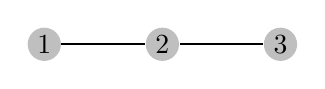
\begin{tikzpicture}[scale=1.5]
    % Draw a 7,11 network
    % First we draw the vertices
    \foreach \pos/\name in {{(1,0)/1}, {(2,0)/2}, {(3,0)/3}}
        \node[vertex] (\name) at \pos {$\name$};
    % Connect vertices with edges 
    \foreach \source/ \dest in {1/2, 2/3}
        \path[edge] (\source) -- (\dest) ;
        
\end{tikzpicture}
\end{center}

If the static game is not to be played repeatedly, one can checked that there is no pure strategy equilibrium which is ex-post efficient if the true state $(t_1,t_2,t_3)=(H,H,H)$\footnote{Player $1$ has been chosen as a high type player. If he choose $h$ then he face the probability of $1-\alpha$ to get pay-off by $-1$ if player $3$ is a $L$ type player. If player $3$ happened to be a $H$ type player (with the probability of $\alpha$), the maximum pay-off player $1$ can get is $1$. But $1-\alpha>\alpha$, choosing $h$ can give him ex-ante pay-off $(1-\alpha)(-1)+\alpha<0$, which is dominated by choosing $l$ which can give him pay-off by $0$. Thus, the only pure strategy Bayesian equilibrium is all players choosing $l$. And this outcome is not ex-post efficient if the true state is $(t_1,t_2,t_3)=(H,H,H)$.}.   

If the static game is to be played repeatedly, we can consider the following strategies and let $\delta\geq \frac{1}{2}$.

\begin{itemize}

\item If a player who is a $L$ type person, he choose $l$ for all period $m$.
\item In the zero period, Player 2 choose $h$ if he observe $t=(H,H,H)$, and keep playing $h$ afterwards. Otherwise, he choose $l$ and keep playing $l$ afterwards. 
\item In the zero period, Player 1 and player 3 choose $l$ no matter what type they are.
\item If player 1 (or player 3) is a $H$ type persons, there are two cases. If Player 2 choose $h$ in the last period, then player 1 (or player 3) keep playing $h$ afterwards; if Player 2 choose $l$ in the last period, then player 1 (or player 3) keep playing $l$ afterwards.
\end{itemize}


The above strategies is to let player 2 to be a coordinator to coordinate player 1 and player 3 if he observe $t=(H,H,H)$. If the true states are other than $(H,H,H)$, since player 2 can observe everyone's type, he will not deviate to play $h$. If the true state is $(H,H,H)$, if he did not deviate, he will get average pay-off $(1-\delta)(-1)+\delta\geq 0$ since $\delta\geq \frac{1}{2}$. But if he deviate, he will get $0$ in current period and still get $0$ afterwards. 

For player 1 (or player 3), at the state $(H,H,H)$, if he deviate in zero period, he at most get ex-ante average pay-off by $\alpha+(1-\alpha)(-1)(1-\delta)=\alpha-(1-\alpha)(1-\delta)$. If he did not deviate, he will get $\alpha\delta+(1-\alpha)0=\alpha\delta$. But $(1-\alpha)>\alpha$, he will not deviate. After zero period, since player 2 play $h$ only if the true state is $(H,H,H)$, if he observe player 2 played $h$, the best response for himself is to keep playing $h$; if he observe player 2 played $l$, he will keep play $l$.

After zero period, if the true state is $(t_1,t_2,t_3)=(H,H,H)$, every player chooses $h$. And if $\delta$ is close to one, the ex-ante pay-off is close to $1$.

\begin{remark}
Note that I put $\alpha<1/2$ as an assumption through out this paper. If $\alpha\geq 1/2$, every player play $h$ is a possible Bayesian equilibrium. Instead of that, I focus on ex-post efficient sequential equilibrium even if this case is impossible.

The static pay-off here is assumed to be hidden. If the pay-off is not hidden, consider the case $G_1=\{1\},G_2=\{2,3\},G_3=\{3,2\}$, and let all players are high types. Although player $1$ is an isolated player, he still can report his type by playing $h$ through the static pay-off. Even if there is no link between $1$ and $2$, $1$ still can transmit relevant signal to $2$. It will let network structure become less important. Instead of that, I focus on the information structure which has been described by network structure. $\blacksquare$
\end{remark}

\subsection{Belief Updating}

By Proposition ~\ref{prop:domi}, the consequence is that, if a $H$ type $i$ play $h$ in some periods, this action will let $i$'s neighbour, says $j\in G_i$ knows that $i$'s another neighbour (if one exists) is not a $L$ type player.

I now give the notations for automation representation first, and then characterize the belief updating induced by the automata.

Let $\{\mathcal{W}_i, \tau_i, f_i, \omega^{0}_i\}_i$ be the automation, $\mathcal{W}_i$ is a finite set of states, $\tau_i: \mathcal{W}_i\times \prod_{-i\in G_i}A_j\rightarrow \mathcal{W}_i$ is the transition function, $f_i: \mathcal{W}_i\rightarrow A_i$ is the output function, and $\omega^{-1}_i: T\rightarrow \mathcal{W}_i$ is the initial state which is itself a measurable function of $t$ with respect to $i$'s information partition $\mathcal{P}_{G_i}$ over $T$. 

At initial period, let $\beta^{\pi,\tau}_{G_i}(t|h^{0}_i)$ be $i$'s belief over players' types $t$ in initial private history $h^{0}_i=\{\emptyset\}$. This initial belief is just the posterior over $T$ given $\pi,G_i$. Define $T_{h^{0}_i}=\{t: (a^1_i,f_{-i\in G_i}(\omega^1_{-i\in G_i}(t)))=(a^1_i,a^1_{-i\in G_i})\}$ be the set of types which can generate $i$'s private history up to first period, and define a indicator function $\mathbb{I}(t\in T_{h^{-1}_i})=1$ if $t\in T_{h^{-1}_i}$; $=0$ if $t\notin T_{h^{-1}_i}$. Then the 
belief $\beta_{G_i}(t|h^1_i)$ is 
\begin{equation}
\label{eqn:updatingini}
\beta_{G_i}(t|h^1_i)=\frac{\beta_{G_i}(t|h^{0}_i)\mathbb{I}(t\in T_{h^{0}_i})}{\sum_{t\in T}\beta_{G_i}(t|h^{0}_i)\mathbb{I}(t\in T_{h^{0}_i})}
\end{equation}

After initial period, at $s$th period, since the arriving state $\omega^s_i$ is determined by $i$'s transition function, and thus it is also a function of $t$. That is, for all $i$, at $s$th period,
\begin{equation}
\omega^s_i(t) =\tau_i(\omega^{s-1}_i, a^{s-1}_i, f_{-i\in G_i}(\omega^{s-1}_{-i\in G_i}(t)))
\end{equation}
. Then define $T_{h^{s-1}_i} = \{t: (a^s_i,f_{-i\in G_i}(\omega^s_{-i\in G_i}(t)))=(a^s_i,a^s_{-i\in G_i})\}$, and define $\mathbb{I}(t\in T_{h^{s-1}_i})$ recursively. The belief $\beta^{\pi, \tau}_{G_i}(t|h^s_i)$ is updating by

\begin{equation}
\label{eqn:updatingend}
\beta_{G_i}(t|h^s_i)=\frac{\beta_{G_i}(t|h^{s-1}_i)\mathbb{I}(t\in T_{h^{s-1}_i})}{\sum_{t\in T}\beta_{G_i}(t|h^{s-1}_i)\mathbb{I}(t\in T_{h^{s-1}_i})}
\end{equation}

Furthermore, if a player $j\neq i$ did not follow his automata, player $i$ form the belief by the following assumption.
\begin{assumption}
\label{assm:notexists}
If $\nexists t\in T_{h^{s-1}_i} $, then $\beta_{G_i}(t|h^s_i)=\beta_{G_i}(t|h^{s-1}_i)$
\end{assumption}

\begin{remark}
The Assumption ~\ref{assm:notexists} is the assumption on beliefs if some players' strategies are outside the equilibrium path. $\blacksquare$
\end{remark}



\section{Main Results}
\label{sec:results}
\subsection{Equilibrium}
In this section, I am finding the sequential equilibrium in some classes of networks, which is approaching ex-post efficient for the game described in last section. I begin with some definition to define the network.

\begin{definition}
A path from $i$ to $j$ in a network $G$ is a finite sequence $k^1,...,k^q$ such that $k^1=i, k^2\in G_{k^1}\backslash k^1, k^3\in G_{k^2}\backslash k^2,...,k^q\in G_j\backslash j$. The shortest path from $i$ to $j$ is the path which has minimum $q$. Called the this minimal $q$ as $q_{ij}$ be the \textit{distance} from $i$ to $j$.
\end{definition}

\begin{definition}
$G$ is connected if and only if for all $i,j$, $i\neq j$, there is a path from $i$ to $j$.
\end{definition}

\begin{definition}
$G$ is crowded if and only if for all $i$, $\# G_i\backslash i\geq 2$
\end{definition}




The graph of a connected crowded or not-crowded network can be seen in Table ~\ref{table_CN_figures}. I also call the players \textit{spike} players if they have only one neighbour; call the players \textit{non-spike} players if they have at least $2$ neighbours.

\begin{proposition}
\label{prop:crowded}
For $\alpha<1/2$, If $G$ is a finite, connected and crowded network, then there is a $\delta_{\alpha}$ and a pure strategy sequential equilibrium if $\delta\geq\delta_{\alpha}$, such that this equilibrium is approaching ex-post efficient.
\end{proposition}

\bigskip
\noindent\underline{\emph{The strategies for Proposition ~\ref{prop:crowded}}}

For each player $i$, there are two private states: $\mathcal{W}_i=\{\omega_{Ll},\omega_{Hh}\}$.  The output function $f(\omega_{e_1e_2})=e_2$.  If $t_i=L$ or there is at least one $j\in G_i$ such that $t_j=L$, the initial state $\omega^0_i=\omega_{LI}$; otherwise $\omega^0_i=\omega_{Hh}$. 

The transition function for $i$ player can be seen in the following figure. 

\begin{center}
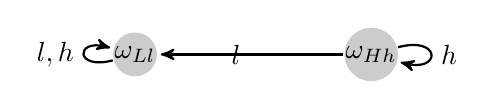
\begin{tikzpicture}[->,>=stealth',shorten >=1pt,auto,node distance=3cm,
  thick,main node/.style={circle,fill=black!20,minimum size=12pt,inner sep=0pt}]

  \node[main node] (1) {$\omega_{Ll}$};
  \node[main node] (2) [right of=1] {$\omega_{Hh}$};

  \path
    (1) edge [loop left] node {$l,h$} (1)
    (2) edge node [left] {$l$} (1)
    edge [loop right] node {$h$} (2);


\end{tikzpicture}
\end{center}
,where the notation $h$ means $h$ is played by all of his neighbours, and $l$ means $l$ is played by one of his neighbours.

\bigskip

\begin{remark}
The logic behind this strategy is that once a player knows that there is a $L$-type player, then he stop playing $h$. Every player will truthfully report his neighbours' type eventually since the network is finite. With high $\delta$, players will not deviate from the equilibrium path. If a player deviate, due to our belief updating Assumption ~\ref{assm:notexists}, the expected continuation pay-off will end up to $0$. However, if he did not deviate, one can show that the expected continuation pay-off is increasing as periods goes by. 

Moreover, note that every player will play $h$ starting from the first period if all the players are $H$ types. $\blacksquare$
\end{remark}



\begin{proposition}
\label{prop:not_crowded}
For $\alpha<1/2$, if $G$ is a a finite connected but not-crowded network, then there is a $\delta_{\alpha}$ and a pure strategy sequential equilibrium if $\delta\geq\delta_{\alpha}$, such that this equilibrium is approaching ex-post efficient.
\end{proposition}

\noindent\underline{\emph{The strategies for spike player in Proposition ~\ref{prop:not_crowded}}}

For spike players $s$, there are three private states, $\mathcal{W}_s=\{\omega_{Ll},\omega_{Hh},\omega_{Hl}\}$.  and the output function $f(\omega_{e_1e_2})=e_2$.  If $t_s=L$ or at least one $j\in G_s$ such that $t_j=L$, the initial state $\omega^0_r=\omega_{LI}$; otherwise $\omega^0_r=\omega_{Hl}$. 

The transition function for spike players can be seen in the following graph. 


\begin{center}
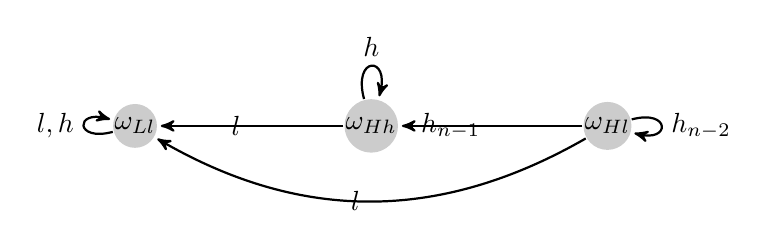
\begin{tikzpicture}[->,>=stealth',shorten >=1pt,auto,node distance=3.0cm,
  thick,main node/.style={circle,fill=black!20,minimum size=12pt,inner sep=0pt}]

  \node[main node] (1) {$\omega_{Ll}$};
  \node[main node] (2) [right of=1] {$\omega_{Hh}$};
  \node[main node] (3) [right of=2] {$\omega_{Hl}$};


  \path
    (1) edge [loop left] node {$l,h$} (1)
    (2) edge node [left] {$l$} (1)
    edge [loop above] node {$h$} (2)
    (3) edge [bend left] node [left] {$l$} (1)
    edge node [left] {$h_{n-1}$} (2)
    edge [loop right] node {$h_{n-2}$} (3);

\end{tikzpicture}
\end{center}
, where the notation $h_{m}$ means action $h$ has been played continuously by his neighbour for $m$ times. The notation $h$ means $h$ is played by all of his neighbours, and $l$ means $l$ is played by one of his neighbours. 

\bigskip

\noindent\underline{\emph{The strategies for non-spike player in Proposition ~\ref{prop:not_crowded}}}

The same as the players in crowded network, expect for the transition function did \textit{not} take account spike players actions.

\bigskip

\begin{remark}
The main difference between crowded and not-crowded network lies on spike players' behaviour. A $H$ type spike player will play $l$ until he knows all other players are $H$ types. Conversely, A $H$ type non-spike player will play $h$ until he knows there is a $L$ type player somewhere. This is mainly because the spike player can \textit{not} transmit further information to other players, and thus other players can not punish him by shifting to worst equilibrium where all players play low inputs\footnote{One may concern whether all players behave like non-spike players is an equilibrium. The answer is it may not, even if the static pay-off itself is a signal. Consider the leading example, and consider player $1$ who has been chosen as $H$ type. By playing $h$ in the first period, he at most get $1$ with probability $\alpha$ if player $2$ and $3$ are all $H$ types and all play $h$ in first period, but get $-1$ with probability $1-\alpha$. Clearly, if $\alpha<1/2$, he will not do so. Indeed, if we allow the static pay-off signal, the true state will be revealed just after first period, but it did not affect first-period behaviour.}. 

In the above equilibrium for not-crowded network, all players will end up to play $h$ if all the players are $H$ types, and end up to play $l$ If there is a $L$ player somewhere. $\blacksquare$
\end{remark}


The last thing is the case if $G$ is not connected. In such case, there must be a pair of players such that there is no path between them, and hence some players actions can not observed by other players. If the static pay-off is hidden, there is no way to reveal the true state to all players. The only equilibrium is that all players play low inputs if $\alpha<1/2$.




\subsection{Optimal Network}
\label{sec:optimal}
From the above discussion, we can conclude that if a network is not connected, the only sequential equilibrium is that all players play low inputs; if a network is connected, with high discounted factor, there is a sequential equilibrium to let ex-post efficient allocation be achieved. However, there are two different kinds of equilibria subject to two different kinds of connected networks, i.e. crowded or non-crowded. Moreover, there are many possible connected networks with a certain number of players $n$ and certain number of links $l$. 

I am meant to ask if a social planner who want to allocate a $n$-players $l$-links network before nature choose a state, which network structure is ex-ante optimal in those equilibria. I only consider the class of connected network, and focus on the social welfare measured by summing all players' ex-ante pay-off given the prior distribution. 

First, I made a program to find all possible $n$-players $l$-links undirected connected networks\footnote{I treat a undirected network as a symmetric adjacency matrix in which every element is taken from $\{0,1\}$. I then use Johnson's algorithm \cite{Johnson1977} (which has been packaged as a MATLAB package) to check if a generated network is a connected network. A necessary condition for  the connectivity of a network is that if a network is connected then its adjacency matrix is irreducible. But I don't use that property since I also need a sufficient condition. More details can be seen in Appendix. When number of players goes up, the computational time growing very fast. Suppose we can find all possible $n$-players $l$-links in $k$ iterations, the problem of $n+1$-players $l+1$-links  should take at least $c(n+1,1)$ times $k$ iterations, where $c(\cdot,\cdot)$ is the combination symbol. I can only gives the optimal network up to $n=8$.}, and then calculate the social welfare for each possible network given prior parameter $\alpha=0.45$ and varied discounted factor $\delta$. The results are shown in Table ~\ref{table_opn} and Table ~\ref{table_ops}. Note that since every player has the same probability be chosen as a low type player, and low type player's pay-off is irrelevant in finding optimal network\footnote{They always play $l$ and get a constant pay-off}, I did not calculate their ex-ante pay-off in social welfare. And the algorithm is shown in the Appendix.

A quick review of the results in Table ~\ref{table_opn} suggests that an optimal network should have enough centrality and symmetry.  And in Table ~\ref{table_ops}, the results shows that not-crowded networks dominate crowded network in social welfare. The followings are the discussions.

In Table ~\ref{table_opn}, we can see that an optimal network should have enough symmetry. This is mainly because our social welfare is ex-ante, and players type is independently drawn from the prior. Notice that, in crowded networks, every player follows the same strategy; in not-crowded network, non-spike players also follows the similar strategy. Therefore, given the discounted factor, in order to let every $H$ player to follow the equilibrium where he take the risk to report his $H$ type neighbours, the network should be symmetric to let every possible $H$ player has the incentive to do so.

The remaining question is why a optimal network seems taking the from symmetry networks. I still do not have a closed from solution, but the answer could be observed by reviewing the continuation pay-off in a crowded networks. In a crowded networks, the ex-ante pay-off for a player $i$ can be derived as 

\begin{eqnarray*}
E(U_i(\tau^{*})|\beta^{\pi,(\tau^{*})}_{G_i}(t|h^{-1}_{G_i}), G)=(1-\alpha)\times 1+\alpha &\times &[(1-\alpha^{n_{i1}})\times -(1-\delta^{1-1})\\
&+&\alpha^{n_{i1}}(1-\alpha^{n_{i2}})\times -(1-\delta^{2-1})\\
&.&\\
&.&\\
&+&\alpha^{n_{i1}}...\alpha^{n_{id_i-1}}(1-\alpha^{n_{id_i}})\times -(1-\delta^{d_i-1})\\
&+&\alpha^{n_{i1}}...\alpha^{n_{id_i-1}}\alpha^{n_{id_i}}]
\end{eqnarray*}
where $n_{id}$ is the total number of players other than $i$ who has distance $d$ from $i$, $d_i$ is the longest distance from $i$ to someone, and which are constrained by $n_{i1}+...+n_{id_i}=n-1$. The terms $(1-\alpha^{n_{i1}})$ means there is a distance-$1$ neighbour whose type is $L$; $\alpha^{n_{i1}}(1-\alpha^{n_{i2}})$ means all distance-$1$ neighbours are $H$ types but there is a distance-$2$ neighbour whose type is $L$;...;and so on. Remind that $H$ type player continue playing $h$ until he find someone is $L$ type in equilibrium, those terms are just the probabilities he could stop taking the risk.

By observing $-(1-\delta^{1-1})>-(1-\delta^{2-1})>...>-(1-\delta^{k-1})$, we basically want a player $i$ could have higher $(1-\alpha^{n_{i1}})$, higher $\alpha^{n_{i1}}(1-\alpha^{n_{i2}})$,..., and so on. From the social planner's view, that means we want higher $\sum_i(1-\alpha^{n_{i1}})$, higher $\sum_i\alpha^{n_{i1}}(1-\alpha^{n_{i2}})$,...,and so on. He try to find a $G$ given $n$-players and $l$-links in order to maximize the following equation,

\begin{eqnarray*}
\sum_i E(U_i(\tau^{*})     |\beta^{\pi,(\tau^{*})}_{G_i}(t|h^{-1}_{G_i}), G)=(1-\alpha)\times 1+\alpha &\times &[\sum_i(1-\alpha^{n_{i1}})\times -(1-\delta^{1-1})\\
&+&\sum_i\alpha^{n_{i1}}(1-\alpha^{n_{i2}})\times -(1-\delta^{2-1})\\
&.&\\
&.&\\
&+&\sum_i\alpha^{n_{i1}}...\alpha^{n_{id_i-1}}(1-\alpha^{n_{id_i}})\times -(1-\delta^{d_i-1})\\
&+&\sum_i\alpha^{n_{i1}}...\alpha^{n_{id_i-1}}\alpha^{n_{id_i}}]
\end{eqnarray*}

Now take a look of this sequences $(\sum_i(1-\alpha^{n_{i1}}), \sum_i\alpha^{n_{i1}}(1-\alpha^{n_{i2}}),...)$ generated by network $G$s. If we define $o_{id}=\sum^d_{j=1} n_{ij}$ for each distance $d$ for player $i$, one can observe that if $\sum^n_{i=1} o_{ik}$ is a fixed integer number and $0<\alpha<1$, the minimum value of $\sum^n_{i=1}\alpha^{o_{ik}}$ should be happened when $o_{1k},...,o_{nk}$ are as close to each other\footnote{Since $\alpha^{o_{ik}}+\alpha^{o_{jk}}\leq \alpha^{o_{ik}-1}+\alpha^{o_{jk}+1}$ if and only if $o_{ik}\leq o_{jk}$, we can adjust $o_{ik}$ and $o_{jk}$ pair-wisely and then achieve the minimum value.}. 

The above observation shows a potential necessary condition in optimal network. It says we should compare the total numbers of shortest distance and its distribution, and then keep comparing such features for longer and longer distances. Note that the distances in a network decide how many periods should a $H$ type player take risks to play $h$, and thus the social welfare mainly affected by such features in a network.  

Let's go back to Table ~\ref{table_opn} again, and focus on not-crowded networks. Compare $n$-players $l$-links network pairs $(n,l)=(8,8)$ and $(8,10)$. The $(8,8)$ not-crowded network has at most five spike players, and that $(8,10)$ has at most four spike players. The results show, if a not-crowded network can allow some spike players, then allowing as much as spike players achieve optimality. This is because, in equilibrium, the spike players did not take any risk. As a consequence, an optimal network should have fewer players who need to take risks, but those risk-taking players has already transmit the information to all players. 

Another important observation is that we can not just add links from optimal $(8,8)$ not-crowded network to achieve optimal $(8,10)$ one. From optimal $(8,8)$ to optimal $(8,10)$, we not only add some links but also remove some other links. This issue will let the task in finding optimal network become much complicated. 

Table ~\ref{table_ops} shows the social welfare. Given discounted factor, we can see that not-crowded networks almost dominate\footnote{Except for $(8,22)$ networks} crowded network in the sense that which give more social welfare, and the required discounted factors are smaller. However, once the discounted factor can sustain equilibrium for both kinds of networks, the crowded networks rise social welfare more quickly with $\delta$. The main reason is that the non-spike players' pay-off growing more quickly than spike players and a crowded network has more non-spike players\footnote{This calculation is straight-forward and so then I omit it.}. 

The last thing is the issue in computation. As previous discussion, in order to compute the optimal $n$-players $l$-links network, we can not just add links. This optimal network-searching procedure will encounter both removing and adding links. The timing to add or remove the links will also let optimal network-searching procedure be a dynamic problem. 



\section{Extension}

In this section, I am finding the sequential equilibrium which is approaching ex-post efficient in a more general version of Threshold game. I then propose an equilibrium in a specific network structure, and give an example to illustrate the equilibrium path in such equilibrium.

\subsection{Threshold game}
\label{sec:thres}
In the above pay-off setting, as in \cite{chwe2000}, a generalization for the above pay-off setting is to let the term $n-1$ as a parameter. As \cite{chwe2000}, call this class of game as the Threshold game with a parameter $k$ ($1\leq k \leq n$) if it satisfies

\bigskip
\noindent \textbf{Threshold Game Conditions}
\begin{enumerate}
\item $u_i(H,h,a_{-i})=1$, if $\#\{j\in -i|a_j=h\}\geq k-1$
\item $u_i(H,h,a_{-i})=-1$, if $\#\{j\in -i|a_j=h\}<k-1$
\item $u_i(H,l,a_{-i})=0$
\item $u_i(L,l,a_{-i})=1$
\item $u_i(L,h,a_{-i})=0$
\end{enumerate}

Note that the game with $k=n$ is just the game has been used in the above model, and the easiest version of this game is to let $k=1$.

The main difficulty in finding the sequential equilibrium lies on the how to transmit the information about every player's type. Remind that each player has only two possible actions, i.e. playing $h$ or $l$ in each period. The equilibrium constructed as Proposition ~\ref{prop:crowded} and Proposition ~\ref{prop:not_crowded} actually take advantage of the threshold $k=n$. In those propositions, if someone observed someone who is playing $l$ instead of playing $h$, he knows that there is someone is $L$ type and knows that the efficient outcome can not be attained. As a consequence, the information carried by actions $h$ or $l$ represents exactly whether efficient outcome can be attained or not. In the general case $1<k<n-1$, however, even though someone knows that there is some $L$-type players, there could be enough $H$-type players to let the coordination success. Since every player only know parts of numbers of $H$-type players, and thus it could be \textit{no} player knows if the efficient outcome can be sustained. 

Another difficulty is players' strategy generally will not only depend on their knowledge about how many $H$-type players in a network, but also on the knowledge about the locations of $H$-type players. The following example illustrate this situation.

\bigskip

\begin{example}

Take the case of the threshold $k=4$, and let the network be a chain. Consider there are $1,...,10$ players located in the following chain, and label their types (after nature chooses them) as


\begin{center}
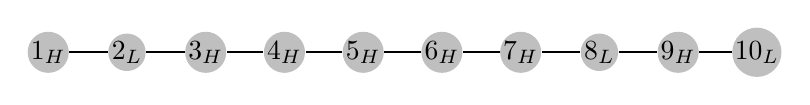
\begin{tikzpicture}[scale=1]
    % Draw a 7,11 network
    % First we draw the vertices
    \foreach \pos/\name in {{(1,0)/1_H}, {(2,0)/2_L}, {(3,0)/3_H}, {(4,0)/4_H}, {(5,0)/5_H}, {(6,0)/6_H}, {(7,0)/7_H},{(8,0)/8_L},{(9,0)/9_H},{(10,0)/10_L}}
        \node[vertex] (\name) at \pos {$\name$};
    % Connect vertices with edges 
    \foreach \source/ \dest in {1_H/2_L, 2_L/3_H,3_H/4_H,4_H/5_H,5_H/6_H,6_H/7_H, 7_H/8_L,8_L/9_H,9_H/10_L}
        \path[edge] (\source) -- (\dest) ;
        
\end{tikzpicture}
\end{center}

For player $3$, he can observed $2$ and $4$'s types at initial period. Different from the strategies described in Section ~\ref{sec:results}, although he know player $2$'s type is $L$, he may not willing to play $l$ at the initial period. This is because he would consider player $4,5,6$ may be all $H$s, and if they followed the same strategies in Section ~\ref{sec:results}, all of they will play $h$ at initial period. Since there will be $k-1=3$ other players play $h$, he is \textit{willing} to deviate to play $h$.

Take a look at player $9$, he may also consider the possibility that there are $k-1=3$ other players play $h$ at the initial period. However, there are no further information can be transmitted to update his belief about other players' types, since his neighbours are $L$ types and they will always play $l$. Thus, player $9$ play $l$ is the dominant strategy if the $\alpha$ is sufficiently small.

Now go back to player $3$. If he consider $4,5,6$ players are in the same situation as player $9$, he will change his mind and is \textit{not willing} to deviate to play $h$.

Combine the above observation, a player will not only consider his neighbours' types, but also need to consider the allocation of the realization of players' types. $\blacksquare$
\end{example}
\bigskip

In order to simplify the analysis, I attempt to make an assumption to rule out the dependency of the locations of the realization. I use Assumption ~\ref{asump_small} on the parameter $\alpha$ to let a $H$-type player playing $h$, no matter how his location is, is \textit{not} a strategy in any Bayesian Nash equilibrium in each of stage games. By using this assumption, in each of stage games, if he is still uncertain whether the total number of $H$-type players excess the threshold, he thinks the probability on this event is very low. Specifically speaking, let $G^H_i=\{j\in G_i|t_j=H\}$ and let $P(n,m)=\sum^n_m c(n,m)\alpha^m(1-\alpha)^{(n-m)}$. For each player $i$, choose a $\bar{\alpha}_i>0$ such that 
\begin{eqnarray*}
1-P(n-\#G^H_i,k-\#G^H_i) &>& P(n-\#G^H_i,k-\#G^H_i) \\
& . &\\
& . &\\
1-P(n-k+1,1) &>& P(n-k+1,1)
\end{eqnarray*}
, where $k-\#G^H_i\geq 1, n>k$ and where $P(n,m)$ is the probability on the event that there are enough amount of $H$-type players which can excess the threshold $k$, conditioning on $i$ is still uncertain about whether the total number of $H$-type players excess the threshold. Since only $H$-type would play $h$ in each stage game, the above equations says to play $h$ is not optimal for him if he simply thinks there are enough high type players in the each stage game. 

The Assumption ~\ref{asump_small} follows.

\begin{assumption}
\label{asump_small}
$\alpha\leq \min \{\bar{\alpha}_1,...,\bar{\alpha}_n\}$
\end{assumption}

\begin{remark}
The Assumption ~\ref{asump_small} is strict in the sense that the $\alpha$ is at most taken as the minimum across $\bar{\alpha}_i$. However, since the goal of this paper is to find the equilibrium which can gives approaching ex-post outcome even if $\alpha$ is low, the result by using this assumption is treated as a partial result. $\blacksquare$
\end{remark}


I now give a pure strategy sequential equilibrium which is approaching ex-post efficient in a loose sense in a specific network. I call this network the \textit{centipedes} network. 

\begin{definition}
A centipedes is a tree in which there is a chain such that all of the spike players connect to some nodes of that chain. Among these chains, pick the longest chain and call such chain the spine of a centipedes. If a player is located on the spine and who is a non-spike player, then call him spine player.
\end{definition}

Figure ~\ref{fig_centi} is an example of a centipedes network. I also assume that the spine of a centipedes is commonly known by all players. 

\begin{assumption}
\label{assum_spine}
The spine of a centipedes is common knowledge.
\end{assumption}

\begin{figure}
\caption{A centipedes}
\label{fig_centi}
\begin{center}
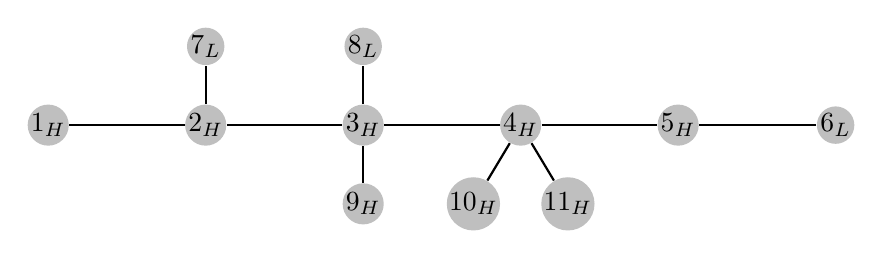
\begin{tikzpicture}[scale=2]
    % Draw a 7,11 network
    % First we draw the vertices
    \foreach \pos/\name in {{(1,1)/1_H}, {(2,1)/2_H}, {(3,1)/3_H}, {(4,1)/4_H}, {(5,1)/5_H}, {(6,1)/6_L}, {(2,1.5)/7_L}, {(3,1.5)/8_L}, {(3,0.5)/9_H}, {(3.7,0.5)/10_H}, {(4.3,0.5)/11_H}}
        \node[vertex] (\name) at \pos {$\name$};
    % Connect vertices with edges 
    \foreach \source/ \dest in {1_H/2_H, 2_H/3_H,3_H/4_H,4_H/5_H,5_H/6_L, 2_H/7_L, 3_H/8_L, 3_H/9_H, 4_H/10_H, 4_H/11_H}
        \path[edge] (\source) -- (\dest) ;
        
\end{tikzpicture}
\end{center}
\end{figure}

\begin{definition} A sequential equilibrium is \textit{approaching ex-post efficient in $\bar{T}\subset T$} if, in all state $t\in \bar{T}$, the stage game outcome is converging to the efficient outcome in the stage game with $T=\{t\}$. \end{definition}

\begin{proposition}
\label{prop_centi}
Suppose Assumption ~\ref{asump_small} ~\ref{assum_spine} hold, the network is finite, centipedes, and in the states such that there is no spine player who is $L$-type after nature choose a state. Then there is a $\delta_{\alpha}$ and a pure strategy sequential equilibrium if $\delta\geq\delta_{\alpha}$, such that this equilibrium is approaching ex-post efficient in those states.
\end{proposition}


\bigskip

\noindent\underline{\emph{The strategies for spike player in a centipedes network}}

A $H$ type spike player will play $l$ until he knows there are at least $k$ other players are $H$ types.

\bigskip

\noindent\underline{\emph{The strategies for a spine player $i$ in a centipedes network}}

\begin{itemize}
\item At the initial period, if he is sure that the total number of $H$-type player is less than threshold, go to Phase \textit{Concluding}. Otherwise, for the players who has two $H$-type spine players as his neighbours, playing $h$ and then go to Phase \textit{Passing}; for the players who has only one spine player as his neighbour, playing $h$ if $\#G^H_i-1>1$ and then go to Phase \textit{Passing} , or playing $l$ if $\#G^H_i-1=1$ and then mimic the strategy as a spike player .

\item Phase \textit{Passing}: If $\#G^H_i-3=0$ and he has only one spine neighbour (other than himself), let $NP=NSR=NSL=0$. Store $NP,NSR,NSL$, play $l$ once and then go to Phase \textit{PassingL} (or \text{PassingR}) dependent on his spine neighbour is on left-handed side (or right-handed side). If $\#G^H_i-3>0$, or $\#G^H_i-3=0$ but he has two spine neighbours, play $h$ until he observe one of spine players playing $l$. Calculate the total number of playing $h$ by his spine-neighbours before he observe one of them playing $l$. Store this number as $NP$. If he only observed right-hand side (or left-hand side) spine player playing $l$, then go to Phase \textit{SendingR} (or \textit{SendingL}); otherwise, go to Phase \textit{Concluding}. 

\item Phase \textit{SendingR(SendingL)}: If $\#G^H_i-3>0$, he first play $h$ for $\#G^H_i-3$ times. Calculate the total number of continuously playing $h$ by left-hand side (or right-hand side) spine player during his own playing $h$. Store this number as $NSR$ (or $NSL$). If $\#G^H_i+NP+NSR($or $NSL)\geq k$, continue playing $h$ afterwards; if $\#G^H_i+NP+NSR($or $NSL)< k$ and left-hand side (right-hand side) spine player play $l$ once during his own playings, go to Phase \textit{Concluding}; if $\#G^H_i+NP+NSR($or $NSL)< k$ and left-hand (right-hand) spine player has not yet played $l$, then he play $l$ once and then go to Phase \textit{PassingL(PassingR)}. If $\#G^H_i-3=0$, store $NSR$(or $NSL$)$=0$, play $l$ once and then go to Phase \textit{PassingL(PassingR)}.


\item Phase \textit{PassingL(PassingR)}: Play $h$ until he observe the left-hand (right-hand) spine players playing $l$. Calculate the total number of playing $h$ by left-hand side (Right-hand side) player before he play $l$, and store this number as $NPL(NPR)$. If $\#G^H_i+NP+NSR($or $NSL)+NPL($or $NPR)\geq k$, continue playing $h$ afterwards; if $\#G^H_i+NP+NSR($or $NSL)+NPL($or $NPR)< k$ then go to Phase \textit{Concluding}. 

\item Phase \textit{Concluding}: Continue playing $l$ afterwards.

\item (Punishment) In any period $\bar{s}>0$, for $H$-type player $i,j$ and $j\in G_i\setminus i$. If $\#\{s\in\{0,...,\bar{s}-1\}|\tau^s_j=h\}+\#\{s\in\{0,...,\bar{s}-1\}|\tau^s_i=h\}\geq k-2$ but $\tau^{\bar{s}}_j=l$, then player $i$ go to Phase \textit{Concluding}.

\end{itemize}

\bigskip

\begin{remark}
The above strategy is to let the spine player transmit the information. The assumption ~\ref{assum_spine} is to let players knows where the information comes from. Along the spine of a centipedes, the spine player play $h$ only if there is still a possibility that the efficient outcome can be sustained. Whenever a spine player observe the right-hand side (or left-hand side) spine player play $h$, he then knows that there is one more $H$-type player on the right-hand side (or left-hand side). The dedicated part is that if he observes a spine player playing $l$. If his right-hand side spine player plays $l$ at the first time, following the above strategy, he immediately knows that there is no more $H$-type players on the right-hand side. In this situation, he starts to reveal the number of spike players who are connected to him by playing $h$. At the same time, he also records how many $H$-type players on the left-hand side. Notice that his own actions can be observed by both of right-hand side and left-hand side members, thus he still transmit the numbers of $H$-type players to his neighbours. After he reveal the types of the spike players, he then play $l$ to let his left-hand side spine player knows that there is no more $H$-type players on the right-hand side. After he plays $l$, he then go back to play $h$ to pass the information from left-hand side to right-hand side. Now although he go back to play $h$, the left-hand side spine player will not be confused to infer his behaviour as there is one more $H$-type player. That is because his left-hand side player has already seen he has been played $l$ before. 

The information flow only through the spine players is crucial here. One can see that there are only two directions to transmit information, i.e. coming from right-hand side or left-hand side. Since there are only two available actions, these two actions essentially play the roles as "opening" the gate (i.e. playing $h$) or as "closing" the gate (i.e. playing $l$) in order to control the information flows. $\blacksquare$
\end{remark}

\bigskip
\begin{example}
Now take an example to make the above strategy more clear. Take a centipedes depicted in Figure ~\ref{fig_centi}. Table ~\ref{eqnpath_thre_8} and Table ~\ref{eqnpath_thre_9} illustrate the equilibrium path for spine players in the $k=8$ Threshold game and $k=9$ Threshold game respectively. The above strategies should let players' actions be coordinated $h$ in the $k=8$ threshold game and to $l$ in the $k=9$ threshold game.

In Table ~\ref{eqnpath_thre_8}, the spine players' actions are coordinated to $h$ after period 6. Player 4 knows there are at least $8$ $H$-types after period 3, and then he continue playing $h$. Since he continues playing $h$, his behaviour will spread over the network. It turns out every $H$ player will play $h$ eventually.

In Table ~\ref{eqnpath_thre_9}, the spine players' actions are coordinated to $l$ after period 6. Player 4 knows there are at least $8$ $H$-types after period 3. However, he observes player 3 and player 5 play $l$ at period 3 and then he knows there is no more $H$-type players on the both sides. He then continue playing $l$. As for Player 3, he observe that player 2 play $l$ at period 2 and player 4 play $l$ at period 4, he will know that there is no more $H$-type players on the both sides after period 4, and then he continue playing $l$. Eventually, the coordination happens after period 6. $\blacksquare$

\end{example}

\bigskip

\begin{table}[tbp]
\caption{Equilibrium path for spine players in Threshold $k=8$ game}
\label{eqnpath_thre_8}
\begin{center}
\begin{tabular}{ccccc}
Periods & Player 2 & Player 3 & Player 4 & Player 5 \\ \hline \hline
0 & $h$ & $h$ & $h$ & $l$\\ 
1 & $l$ & $h$ & $h$ & $l$\\ 
2 & $h$ & $h$ & $h$ & $l$\\ 
3 & $h$ & $h$ & $h$ & $l$\\ 
4 & $h$ & $h$ & $h$ & $l$\\ 
5 & $h$ & $h$ & $h$ & $l$\\ 
6 & $h$ & $h$ & $h$ & $h$\\ \hline \hline
\end{tabular}
\end{center}
\end{table}

\begin{table}[tbp]
\caption{Equilibrium path for spine players in Threshold $k=9$ game}
\label{eqnpath_thre_9}
\begin{center}
\begin{tabular}{ccccc}
Periods & Player 2 & Player 3 & Player 4 & Player 5 \\ \hline \hline
0 & $h$ & $h$ & $h$ & $l$\\ 
1 & $l$ & $h$ & $h$ & $l$\\ 
2 & $h$ & $h$ & $h$ & $l$\\ 
3 & $h$ & $l$ & $h$ & $l$\\ 
4 & $h$ & $h$ & $l$ & $l$\\ 
5 & $h$ & $l$ & $l$ & $l$\\ 
6 & $l$ & $l$ & $l$ & $l$\\ \hline \hline

\end{tabular}
\end{center}
\end{table}
















\section{Conclusion}
\label{sec:con}

Which individuals can be coordinators to guide the whole society to an efficient outcome depends on the location of such individual. From example, in a not-crowded network, the non-spike players are coordinators; in a centipedes, the spine players play such roles. Since network is commonly known, individuals can know where are those coordinators and trace the information flow along with the network. Especially, in a not-crowded network in Section ~\ref{sec:results}, everyone is a coordinator. Combine the above results, if one want to relax the common knowledge assumption, says the game being played in a random network, the analysis have to consider the uncertainty about individuals' allocation and their role to transmit the information. 

To change a network also means to change the initial information about the true state in this model. This feature may link the existing Graph Theory literature to analyze how incomplete information affects in repeated game (such as \cite{sorin1996}).  We may also think a inhabitant can strategically form the link to others, so that they can gather information aggressively. That is to combine the result in network formation literature \cite{JAsurvey2003} and the literature in incomplete information repeated game, then to understand the dynamic information aggregation.

\bibliographystyle{abbrvnat}	% (uses file "plain.bst")
\bibliography{3_rd_refs}		% expects file "myrefs.bib"


\appendix



\section{Proofs}
\subsection{proof of Proposition ~\ref{prop:domi}}
\begin{proof}
If this $H$ type $i$ player deviate in some periods from playing $l$ to playing $h$, then he get $-1$ in those period since there is a player play $l$ in those periods. However, playing $l$ can give him pay-off $0$. That makes him strictly better. 
\end{proof}


\subsection{proof of Proposition ~\ref{prop:crowded}}
\begin{proof}

Given a $H$ type player $i$. For all $j\neq i$, denote $q_{ij}$ be the distance from $i$ to $j$. Denote $q_i=\max_{j}\{q_{ij}\}$. At initial period, clearly, if $\exists j\in G_i,t_j=L$, he should play $l$ forever by Proposition ~\ref{prop:domi}. If not, his automata gives him 
\begin{equation}
\label{eq:crowded}
E(U_i(\tau)|\beta^{\pi,\tau}_{G_i}(t|h^0_{G_i}), G)>(1-\alpha^{n-\# G_i})(-1(1-\delta^{q_i}))+\alpha^{n-\# G_i}
\end{equation}

The term $(-1(1-\delta^{q_i+1}))$ is the continuation pay-off if there is a player in the distance $q_i$ is $L$ type, while all players in the distance less than $q_i$ are all $H$ types.

If he deviates from playing $h$ to play $l$ in some periods, since $G$ is connected, there is a $j,j\neq i$ player play $l$ in all periods. Thus he should play $l$ in all periods and the pay-off end up to zero. We can choose a $\delta_{\alpha}$ to let the right-side terms in Equation ~\ref{eq:crowded} larger than zero, and then he will not deviate given the initial belief. 

Now consider he is in a $s$th period after initial period. There are two cases.

In the case of $\exists t\in T_{h^{s-1}_i}$, if he observed his neighbours play $h$ continuously for $s$ times, he assigned probability one to $t_j=H$ if $q_{ij}\leq s$. The probability on the event that all players are $H$s is increasing in $s$, and so that $E(U_i(\tau)|\beta^{\pi,\tau}_{G_i}(t|h^{s-1}_{G_i}), G)\geq...\geq E(U_i(\tau)|\beta^{\pi,\tau}_{G_i}(t|h^{-1}_{G_i}), G)$. Given the $\delta_{\alpha}$ which has been chosen at initial period, he should follow his automata or he will get continuation pay-off end up to zero. Conversely, if he observed his neighbours play $l$ once, he knows that there is a $L$ player somewhere, and then he should keep playing $l$.

In the case of $\nexists t\in T_{h^{s-1}_i}$, he did not update his belief by Assumption ~\ref{assm:notexists}. However, If he observed one of his neighbours play $l$, since there is another player will play $l$ (i.i the players who share the same neighbour with him), and since the network is connected, there is a $j,j\neq i$ play $l$ in all periods. And then he should always play $l$. The other case is that he observed all of his neighbours play $h$. In this case, since he did not update his belief, he follow the strategy as in the previous period. 

Clearly, if $T=\{t\}=\{H,H,...,H\}$, this automata gives ex-post efficient allocation since all players play $h$ starting from the initial period. If the state is other than all players are $H$ types, all players end up to play $l$ in finite periods since our network is finite.

\end{proof}


\subsection{proof for Proposition ~\ref{prop:not_crowded}}
\begin{proof}

We only consider the case with $n\geq 3$ and the numbers of links number $l> n$\footnote{If $l=n$, the argument is the same as the leading example, and then I omit it. If $l<n$, there is no connected network}. This proof will only consider spike players, since the proof for non-spike players is exact the same as the players in crowded network\footnote{Except for the expected continuation pay-off in Equation ~\ref{eq:crowded} for non-spike player $j$ should be $E(U_i(\tau)|\beta^{\pi,\tau}_{G_j}(t|h^0_{G_j}), G)>(1-\alpha^{n-\# G_j})(-1(1-\delta^{q_j}))+\alpha^{n-\# G_i}(-1(1-\delta^{q-1})+\delta^{q-1})$, where $q$ is the \textit{diameter} (i.e. the longest distance between all players in a network $G$) in a connected network}. 

Given a $H$ type spike player $i$. For all $j\neq i$, denote $q_{ij}$ be the distance from $i$ to $j$. Denote $q_i=\max_{j}\{q_{ij}\}$\footnote{Actually, for all spike players this $q_i$ is constant, which is equal to the \textit{diameter} in a network.}. At initial period, clearly, if $\exists j\in G_i, t_j=L$, he should always play $l$ forever by Proposition ~\ref{prop:domi}. If not, his automata gives him 
\[
E(U_i(\tau)|\beta^{\pi,\tau}_{G_i}(t|h^0_{G_i}), G) = \alpha^{n-2}\delta^{q_{i}-1}
\]

If he deviates his automata from playing $l$ to $h$ in some periods $s=0,...,q_{i}-1$, since he still face uncertainty about the players outside the distance $s$ and $\alpha<1/2$, he get positive loss due to this uncertainty. Furthermore, since the other players did not take account of his actions, he should continue playing $l$.

After he continuously observed $h$ for $q_{i}-1$ times, he assign probability one to the event that all players are $H$ types, and then he should play $h$ afterward.

Combine the spike players' strategies and non-spike players' strategies, after $q_{i}-1$th period, all player play $h$ in the true state $t=(H,...,H)$. If the state is other than all players are $H$ types, all players end up to play $l$ in finite periods since our network is finite.

\end{proof}

\subsection{proof for Proposition ~\ref{prop_centi}}
\begin{proof}

First, if players follow the equilibrium path, to show that these strategies is approaching ex-post efficient is straightforward. I then show these strategies constitute a pure strategy sequential equilibrium.

For a spike player, the proof is the same for the spike players in the non-crowded network for $k=n$ game and so that I omit it. For a spine player, if at some periods he deviates from $h$ to $l$, there is a spine player (i.e. his right-hand side or left-hand side spine player) will believe that there is no more $H$-type players comes from his side by the belief updating process and Assumption ~\ref{assm:notexists}. Suppose in the true state there are $\bar{k}\geq k$ $H$-type players, once he deviates from $h$ to $l$, there is a spine player whose knowledge about the total number of $H$-players is strictly less than $\bar{k}$. Therefore, there is a probability that the coordination would end up to playing $l$ instead of to playing $h$. Thus, he will not deviate.

Next, consider if a spine player deviates from $l$ to $h$. According to the belief updating process, once he play $h$, his spine neighbour will know that there is one more $H$-type player comes from his side, and therefore there is a probability, denoted as $q$, on the event that his spine neighbour will end up to play $h$ although the total number of $H$-type players is less than the threshold $k$. Conditional on this event, his expected continuation pay-off will be strictly less since the total number of $H$-type players is less than the threshold. There is also a probability, denoted as $q'$, on the event that his spine neighbour will end up to play $h$ and the total number of $H$-type players excesses the threshold $k$. In this event, he maybe able to let the coordination to play $h$ happen earlier. Now take the $\delta$ sufficient large so that he will not deviate. Furthermore, since $q<q'$ by Assumption ~\ref{asump_small}, he will have positive expected static loss once he deviate.
\end{proof}


\section{Algorithm to find all possible $(n,l)$ undirected connected network}
Take $(3,3)$ as an example, a possible undirected connected network is $G=\{G_1=\{1,2\},G_2=\{2,3\},G_3=\{3,1\}\}$ and its correspondent adjacency is
\[
\left( {\begin{array}{ccc}
 1 & 1 & 1 \\
 1 & 1 & 1\\
 1 & 1 & 1
 \end{array} } \right)
\]

That is we index $1$ in column $i$ and row $j$ if $j$ is $i$'s neighbours.

Now I show the algorithm. First, open a $n\times n$ matrix where the diagonal is $1$. Since my network is undirected, focus on upper triangle matrix only. Given $(n,l)$, we can generate a possible $\#G=\{\#G_1,...,\#G_n\}$ where $\#G_i$ means the number of $i$'s neighbours, and $\sum^n_{i=1}\#G_i=2l+n$.
\begin{enumerate}
\item Starting from player $1$. Find all possible $\#G_1$ members from $\{2,...,n\}$. Take a possible combination. This combination indicates player $1$'s current neighbours\footnote{other than himself}. And then, we get the first column in adjacency matrix. Restore player $1$'s all possible neighbours as $G_1$.
\item If player $i$'s all possible neighbours has been stored, for all $j\neq i$, update $\#G_j$ as $\#G_{j}=\#G_{j}- 1$ if $j\in G_{i}$; otherwise $\#G_{j}=\#G_{j}$. That is, we calculate the remaining number of neighbours $j$ has.
\item Go to player $i+1$. Find all possible $\# G_{i+1}$ members from $\{j\in \{i+1,...,n\}|\#G_j>1\}$. And then we get the $i+1$th column in adjacency matrix. Restore player $i+1$'s all possible neighbours as $G_{i+1}$.
\item Continue this process until $n$th player, and then we get a possible $(n,l)$-network.
\item After we get a possible network, check if this network is connected by checking the all-pair shortest paths is finite (by using Johnson's algorithm).
\item After we get a possible network, given the current updated $\{\#G_1,...\#G_n\}$ and stored $\{G_1,...,G_n\}$, go back to check if $n$th player's all possible neighbours has been considered. If the answer is yes, staring from $n-1$th player and use the next possible combination which has been restore in $G_{n-1}$; if no, check the next possible neighbours for $n$th player.
\item If $i$th player's all possible neighbours has been considered, staring from $i-1$th player and use the next possible combination which has been store in $G_{i-1}$; if not, check the next possible neighbours for $i$th player.
\end{enumerate}



\section{Tables}

\begin{table}[htbp]
\caption{Connected Networks}
\label{table_CN_figures}
\begin{center}
\begin{tabular}{cc}
Crowded & not-Crowded\\ 
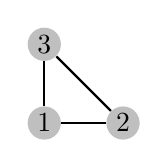
\begin{tikzpicture}[scale=1]
    % Draw a 7,11 network
    % First we draw the vertices
    \foreach \pos/\name in {{(1,1)/1}, {(2,1)/2}, {(1,2)/3}}
        \node[vertex] (\name) at \pos {$\name$};
    % Connect vertices with edges 
    \foreach \source/ \dest in {1/2, 1/3, 2/3}
        \path[edge] (\source) -- (\dest) ;
        
\end{tikzpicture}
&

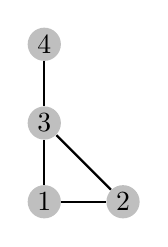
\begin{tikzpicture}[scale=1]
    % Draw a 7,11 network
    % First we draw the vertices
    \foreach \pos/\name in {{(1,1)/1}, {(2,1)/2}, {(1,2)/3},{(1,3)/4}}
        \node[vertex] (\name) at \pos {$\name$};
    % Connect vertices with edges 
    \foreach \source/ \dest in {1/2, 1/3, 2/3,3/4}
        \path[edge] (\source) -- (\dest) ;
        
\end{tikzpicture}
 
\end{tabular}
\end{center}
\end{table}

\begin{table}[htbp]
\caption{optimal network}
\label{table_opn}
\begin{center}
\begin{tabular}{ccc}
 &  & \\  
(n,l) & nCrowded & Crowded\\ \hline \hline
 (7,7)  &  & \\ 
& 
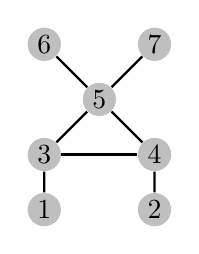
\begin{tikzpicture}[scale=0.7]
    % First we draw the vertices
    \foreach \pos/\name in {{(2,1)/1}, {(4,1)/2}, {(2,2)/3}, {(4,2)/4}, {(3,3)/5}, {(2,4)/6}, {(4,4)/7}}
       \node[vertex] (\name) at \pos {$\name$};
    % Connect vertices with edges 
    \foreach \source/ \dest in {1/3, 2/4, 3/4, 3/5, 4/5, 5/6, 5/7}
        \path[edge] (\source) -- (\dest) ;
\end{tikzpicture}


&


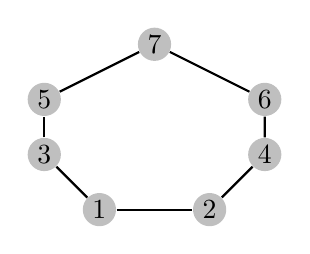
\begin{tikzpicture}[scale=0.7]
    % First we draw the vertices
    \foreach \pos/\name in {{(2,1)/1}, {(4,1)/2}, {(1,2)/3}, {(5,2)/4}, {(1,3)/5}, {(5,3)/6}, {(3,4)/7}}
        \node[vertex] (\name) at \pos {$\name$};
    % Connect vertices with edges 
    \foreach \source/ \dest in {1/2, 1/3, 2/4, 3/5, 5/7, 4/6, 6/7}
        \path[edge] (\source) -- (\dest) ;
\end{tikzpicture}
\\ \hline
(7,11)   &  & \\  
& 
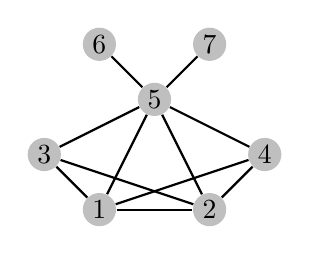
\begin{tikzpicture}[scale=0.7]
    % First we draw the vertices
    \foreach \pos/\name in {{(2,1)/1}, {(4,1)/2}, {(1,2)/3}, {(5,2)/4}, {(3,3)/5}, {(2,4)/6}, {(4,4)/7}}
        \node[vertex] (\name) at \pos {$\name$};
    % Connect vertices with edges 
    \foreach \source/ \dest in {1/2, 1/3, 1/4, 1/5, 2/3, 2/4, 2/5, 3/5,4/5,5/6,5/7}
        \path[edge] (\source) -- (\dest) ;
\end{tikzpicture}


&


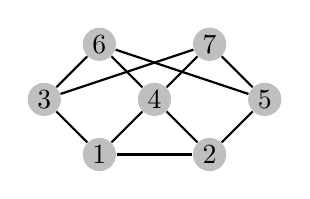
\begin{tikzpicture}[scale=0.7]
    % First we draw the vertices
    \foreach \pos/\name in {{(2,1)/1}, {(4,1)/2}, {(1,2)/3}, {(3,2)/4}, {(5,2)/5}, {(2,3)/6}, {(4,3)/7}}
        \node[vertex] (\name) at \pos {$\name$};
    % Connect vertices with edges 
    \foreach \source/ \dest in {1/2, 1/3, 1/4, 2/4, 2/5, 3/6, 3/7, 4/6,4/7,5/6,5/7}
        \path[edge] (\source) -- (\dest) ;
\end{tikzpicture}
\\ \hline
(8,8)   &  & \\ 
&  
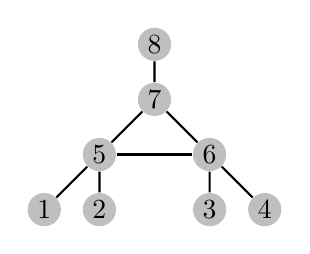
\begin{tikzpicture}[scale=0.7]
    % First we draw the vertices
    \foreach \pos/\name in {{(1,1)/1}, {(2,1)/2}, {(4,1)/3}, {(5,1)/4}, {(2,2)/5}, {(4,2)/6}, {(3,3)/7},{(3,4)/8}}
        \node[vertex] (\name) at \pos {$\name$};
    % Connect vertices with edges 
    \foreach \source/ \dest in {1/5, 2/5, 3/6, 4/6, 5/6, 5/7, 6/7, 7/8}
        \path[edge] (\source) -- (\dest) ;
\end{tikzpicture}

&

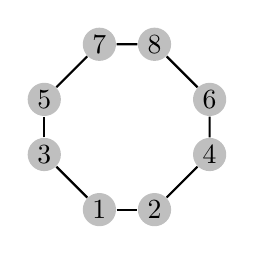
\begin{tikzpicture}[scale=0.7]
    % First we draw the vertices
    \foreach \pos/\name in {{(2,1)/1}, {(3,1)/2}, {(1,2)/3}, {(4,2)/4}, {(1,3)/5}, {(4,3)/6}, {(2,4)/7},{(3,4)/8}}
        \node[vertex] (\name) at \pos {$\name$};
    % Connect vertices with edges 
    \foreach \source/ \dest in {1/2, 1/3, 2/4, 3/5, 4/6, 5/7, 6/8, 7/8}
        \path[edge] (\source) -- (\dest) ;
\end{tikzpicture}

\\ \hline
(8,10)  &  & \\ 
 &  
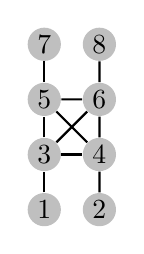
\begin{tikzpicture}[scale=0.7]
    % First we draw the vertices
    \foreach \pos/\name in {{(1,1)/1}, {(2,1)/2}, {(1,2)/3}, {(2,2)/4}, {(1,3)/5}, {(2,3)/6}, {(1,4)/7},{(2,4)/8}}
        \node[vertex] (\name) at \pos {$\name$};
    % Connect vertices with edges 
    \foreach \source/ \dest in {1/3, 2/4, 3/4, 3/5, 3/6, 4/5, 4/6, 5/6,5/7,6/8}
        \path[edge] (\source) -- (\dest) ;
\end{tikzpicture}

&

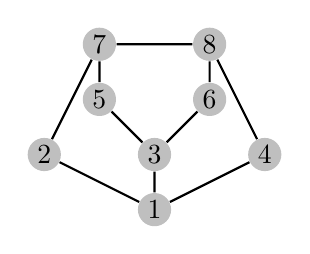
\begin{tikzpicture}[scale=0.7]
    % First we draw the vertices
    \foreach \pos/\name in {{(3,1)/1}, {(1,2)/2}, {(3,2)/3}, {(5,2)/4}, {(2,3)/5}, {(4,3)/6}, {(2,4)/7},{(4,4)/8}}
        \node[vertex] (\name) at \pos {$\name$};
    % Connect vertices with edges 
    \foreach \source/ \dest in {1/2, 1/3, 1/4, 2/7, 3/5, 3/6, 4/8, 5/7,6/8,7/8}
        \path[edge] (\source) -- (\dest) ;
\end{tikzpicture}

 \\ \hline
 (8,13)   &  & \\ 
& 
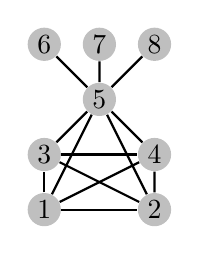
\begin{tikzpicture}[scale=0.7]
    % First we draw the vertices
    \foreach \pos/\name in {{(1,1)/1}, {(3,1)/2}, {(1,2)/3}, {(3,2)/4}, {(2,3)/5}, {(1,4)/6}, {(2,4)/7},{(3,4)/8}}
        \node[vertex] (\name) at \pos {$\name$};
    % Connect vertices with edges 
    \foreach \source/ \dest in {1/2, 1/3, 1/4, 1/5, 2/3, 2/4, 2/5, 3/4,3/5,4/5,5/6,5/7,5/8}
        \path[edge] (\source) -- (\dest) ;
\end{tikzpicture}

&

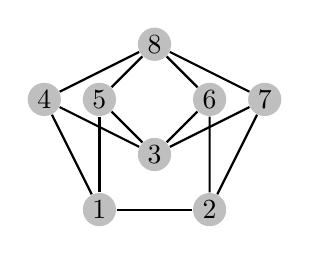
\begin{tikzpicture}[scale=0.7]
    % First we draw the vertices
    \foreach \pos/\name in {{(2,1)/1}, {(4,1)/2}, {(3,2)/3}, {(1,3)/4}, {(2,3)/5}, {(4,3)/6}, {(5,3)/7},{(3,4)/8}}
        \node[vertex] (\name) at \pos {$\name$};
    % Connect vertices with edges 
    \foreach \source/ \dest in {1/2, 1/4, 1/5, 2/6, 2/7, 3/4, 3/5, 3/6,3/7,4/8,5/8,6/8,7/8}
        \path[edge] (\source) -- (\dest) ;
\end{tikzpicture}

\\ \hline
  &  & \\ \hline \hline
\multicolumn{3}{l}{note: In this table $\alpha=0.45$. The optimal network is the same for $\delta\geq 0.95$}\\
\multicolumn{3}{l}{note: nCrowded means not-crowded}
\end{tabular}
\end{center}
\end{table}


\begin{table}[htbp]
\caption{social welfare}
\label{table_ops}
\begin{tabular}{lrcccccc}
&  &  &  &  &  &  & \\ 
($n$,$l$) 	&  & $\delta=0.95$ & $\delta=0.96$ & $\delta=0.97$ & $\delta=0.98$ & $\delta=0.99$ & $\delta=1$\\ \hline\hline
 		&  &  &  &  &  &  & \\ 
(7,7)	 & nCrowded & 0.040 & 0.047 & 0.048 & 0.051 & 0.055 & 0.058\\ 
 		& Crowded & - & - & 0.011 & 0.027 & 0.042 & 0.058\\ 
(7,11) & nCrowded & 0.042 & 0.045 & 0.048 & 0.052 & 0.055 & 0.058\\ 
 & Crowded & 0.032 & 0.037 & 0.042 & 0.048 & 0.053 & 0.058\\ \hline
 &  &  &  &  &  &  & \\ 
(8,8) & nCrowded & - & - & 0.023 & 0.025 & 0.028 & 0.030\\ 
 & Crowded & - & - & - & - & 0.011 & 0.030\\ 
(8,10) & nCrowded & - & - & - & 0.018 & 0.028 & 0.030\\ 
 & Crowded & - & - & - & - & 0.018 & 0.030\\ 
(8,13) & nCrowded & 0.020 & 0.022 & 0.024 & 0.026 & 0.028 & 0.030\\ 
 & Crowded & - & 0.006 & 0.012 & 0.018 & 0.024 & 0.030\\ \hline
  &  &  &  &  &  &  & \\ 
(8,17) & nCrowded & 0.024 & \cellcolor{Gray} & \cellcolor{Gray}  & \cellcolor{Gray} & \cellcolor{Gray} & \cellcolor{Gray}\\ 
 & Crowded & 0.017 & \cellcolor{Gray} & \cellcolor{Gray} & \cellcolor{Gray} & \cellcolor{Gray} & \cellcolor{Gray}\\ 
(8,22) & nCrowded & 0.026 & \cellcolor{Gray} & \cellcolor{Gray} & \cellcolor{Gray} & \cellcolor{Gray} & \cellcolor{Gray}\\ 
 & Crowded & 0.026 & \cellcolor{Gray} & \cellcolor{Gray} & \cellcolor{Gray} & \cellcolor{Gray} & \cellcolor{Gray}\\ 
(8,24) & Crowded & 0.028 & \cellcolor{Gray} & \cellcolor{Gray} & \cellcolor{Gray} & \cellcolor{Gray} & \cellcolor{Gray}\\ 
(8,26) & Crowded & 0.029 & \cellcolor{Gray} & \cellcolor{Gray} & \cellcolor{Gray} & \cellcolor{Gray} & \cellcolor{Gray}\\ 
(8,28) & Crowded & 0.030 & \cellcolor{Gray} & \cellcolor{Gray} & \cellcolor{Gray} & \cellcolor{Gray} & \cellcolor{Gray}\\ \hline
 &  &  &  &  &  &  & \\ \hline \hline
 \multicolumn{8}{l}{note: In this table $\alpha=0.45$. The grey regions means I omit the result.}\\
 \multicolumn{8}{l}{note: The sign "$-$" means the chosen $\delta$ can not sustained the equilibrium I proposed.}\\
  \multicolumn{8}{l}{note: nCrowded means not-crowded}
\end{tabular}
\end{table}


\end{document}
